%%%%%%%%%%%%%%%%%%%%%%%%%%%%%%%%%%%%%%%%%
% Short Sectioned Assignment
% LaTeX Template
% Version 1.0 (5/5/12)
%
% This template has been downloaded from:
% http://www.LaTeXTemplates.com
%
% Original author:
% Frits Wenneker (http://www.howtotex.com)
%
% License:
% CC BY-NC-SA 3.0 (http://creativecommons.org/licenses/by-nc-sa/3.0/)
%
%%%%%%%%%%%%%%%%%%%%%%%%%%%%%%%%%%%%%%%%%

%----------------------------------------------------------------------------------------
%	PACKAGES AND OTHER DOCUMENT CONFIGURATIONS
%----------------------------------------------------------------------------------------

\documentclass[paper=a4, fontsize=11pt]{scrartcl} % A4 paper and 11pt font size

\usepackage{graphicx}
\usepackage[T1]{fontenc} % Use 8-bit encoding that has 256 glyphs
\usepackage{fourier} % Use the Adobe Utopia font for the document - comment this line to return to the LaTeX default
\usepackage[english]{babel} % English language/hyphenation
\usepackage{amsmath,amsfonts,amsthm} % Math packages

\usepackage{lipsum} % Used for inserting dummy 'Lorem ipsum' text into the template
\usepackage{algorithm}
\usepackage{algpseudocode}
\usepackage{sectsty} % Allows customizing section commands
\allsectionsfont{\scshape} % Make all sections centered, the default font and small caps

\usepackage{mathtools}
\usepackage{blkarray, bigstrut} %

\usepackage{algorithm,algpseudocode}% http://ctan.org/pkg/{algorithms,algorithmx}
\algnewcommand{\Inputs}[1]{%
  \State \textbf{Inputs:}
  \Statex \hspace*{\algorithmicindent}\parbox[t]{.8\linewidth}{\raggedright #1}
}
\algnewcommand{\Initialize}[1]{%
  \State \textbf{Initialize:}
  \Statex \hspace*{\algorithmicindent}\parbox[t]{.8\linewidth}{\raggedright #1}
}

\usepackage{fancyhdr} % Custom headers and footers
\pagestyle{fancyplain} % Makes all pages in the document conform to the custom headers and footers
\fancyhead{} % No page header - if you want one, create it in the same way as the footers below
\fancyfoot[L]{} % Empty left footer
\fancyfoot[C]{} % Empty center footer
\fancyfoot[R]{\thepage} % Page numbering for right footer
\renewcommand{\headrulewidth}{0pt} % Remove header underlines
\renewcommand{\footrulewidth}{0pt} % Remove footer underlines
\setlength{\headheight}{13.6pt} % Customize the height of the header

\numberwithin{equation}{section} % Number equations within sections (i.e. 1.1, 1.2, 2.1, 2.2 instead of 1, 2, 3, 4)
\numberwithin{figure}{section} % Number figures within sections (i.e. 1.1, 1.2, 2.1, 2.2 instead of 1, 2, 3, 4)
\numberwithin{table}{section} % Number tables within sections (i.e. 1.1, 1.2, 2.1, 2.2 instead of 1, 2, 3, 4)

\setlength\parindent{0pt} % Removes all indentation from paragraphs - comment this line for an assignment with lots of text

%----------------------------------------------------------------------------------------
%	TITLE SECTION
%----------------------------------------------------------------------------------------

\newcommand{\horrule}[1]{\rule{\linewidth}{#1}} % Create horizontal rule command with 1 argument of height

\title{	
\normalfont \normalsize
\textsc{Rice University, Department of Computer Science} \\ [25pt] % Your university, school and/or department name(s)
\horrule{0.5pt} \\[0.4cm] % Thin top horizontal rule
\huge Assignment 6, COMP 540 \\ % The assignment title
\horrule{2pt} \\[0.5cm] % Thick bottom horizontal rule
}

\author{Chen Zeng(cz39), Zhihui Xie(zx18)} % Your name

\date{\normalsize\today} % Today's date or a custom date

\begin{document}

\maketitle % Print the title

\section{Hidden Markov Models}
\paragraph{\textbf{Answer1}}
Formulate this problem as a Hidden Markov model as below:
\\ The set of observables: $O=\left \{ l, m, h \right \}$, low, medium, or high
\\ The set of hidden states: $S=\left \{ H, U \right \}$, healthy or unhealthy
\\ The parameters $\lambda =\left [ \pi ,a,b \right ]$: 
\begin{itemize}
  \item The initial state distribution: $\lambda :\left [ 0.5, 0.5 \right ]$
  \item The transition matrix: 
	$ \mathbf{a}=
 	 \begin{blockarray}{*{2}{c} l}
    	\begin{block}{*{2}{>{$\footnotesize}c<{$}} l}
     	 H & U & \\
   	 \end{block}
   	 \begin{block}{[*{2}{c}]>{$\footnotesize}l<{$}}
      	0.8 & 0.2 & H \\
      	0.2 & 0.8 & U \\
    	\end{block}
  	\end{blockarray}$
  \item The emission matrix:
	 $\mathbf{b}=
 	 \begin{blockarray}{*{3}{c} l}
    	\begin{block}{*{3}{>{$\footnotesize}c<{$}} l}
     	 l & m & h &\\
   	 \end{block}
   	 \begin{block}{[*{3}{c}]>{$\footnotesize}l<{$}}
      	0.5 & 0.3 & 0.2 & H \\
      	0.3 & 0.3 & 0.4 & U \\
    	\end{block}
  	\end{blockarray}$
\end{itemize}
The corresponding graphical model: please help to refer to figure \ref{fig:markov}
\begin{figure}[H]
 	\centering
 	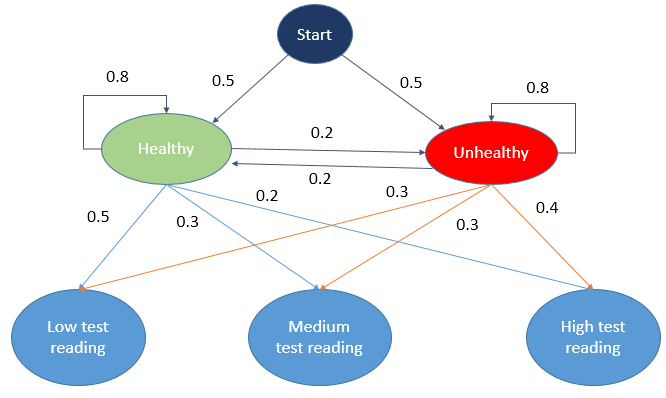
\includegraphics[scale=0.5]{./markov.png}
 	\caption{Markov Chain}
 	\label{fig:markov}
 \end{figure}

\paragraph{\textbf{Answer2}}
\begin{align*}
P\left ( S_{1}=H \right )=P\left ( S_{0}=H \right )P\left ( S_{1}=H|S_{0}=H \right )+P\left ( S_{0}=U\right )P\left ( S_{1}=H|S_{0}=U \right )=0.5*0.8+0.5*0.2=0.5
\end{align*}
\begin{align*}
P\left ( S_{1}=U \right )=P\left ( S_{0}=H \right )P\left ( S_{1}=U|S_{0}=H \right )+P\left ( S_{0}=U\right )P\left ( S_{1}=U|S_{0}=U \right )=0.5*0.2+0.5*0.8=0.5
\end{align*}
\begin{align*}
P=&P\left ( S_{2}=H|O_{1}=l,O_{2}=l \right )
\\=&\frac{P\left ( S_{2}=H,O_{1}=l,O_{2}=l \right )}{P\left ( O_{1}=l,O_{2}=l \right )}
\\=&\frac{P\left ( S_{2}=H,O_{1}=l,O_{2}=l | S_{1}=H \right )P\left ( S_{1}=H \right )+P\left ( S_{2}=H,O_{1}=l,O_{2}=l | S_{1}=U \right )P\left ( S_{1}=U \right )}{P\left ( O_{1}=l,O_{2}=l | S_{1}=H \right )P\left ( S_{1}=H \right )+P\left ( O_{1}=l,O_{2}=l | S_{1}=U \right )P\left ( S_{1}=U \right )}
\\=&\frac{P\left ( S_{2}=H,O_{1}=l,O_{2}=l | S_{1}=H \right )+P\left ( S_{2}=H,O_{1}=l,O_{2}=l | S_{1}=U \right )}{P\left ( O_{1}=l,O_{2}=l | S_{1}=H \right )+P\left ( O_{1}=l,O_{2}=l | S_{1}=U \right )}
\end{align*}
We know that $O_{1}$ is independent to both $S_{1}$ and $O_{2}$, so we have:
\begin{align*}
P\left ( S_{2}=H,O_{1}=l,O_{2}=l | S_{1}=H \right ) = P\left ( S_{2}=H,O_{2}=l | S_{1}=H \right )P\left ( O_{1}=l | S_{1}=H \right )
\end{align*}
\begin{align*}
P\left ( S_{2}=H,O_{1}=l,O_{2}=l | S_{1}=U \right ) = P\left ( S_{2}=H,O_{2}=l | S_{1}=U \right )P\left ( O_{1}=l | S_{1}=U \right )
\end{align*}
Then we have:
\begin{align*}
P=&\frac{P\left ( S_{2}=H,O_{2}=l | S_{1}=H \right )P\left ( O_{1}=l | S_{1}=H \right )+P\left ( S_{2}=H,O_{2}=l | S_{1}=U \right )P\left ( O_{1}=l | S_{1}=U \right )}{P\left ( O_{1}=l | S_{1}=H \right )P\left ( O_{2}=l | S_{1}=H \right )+P\left ( O_{1}=l | S_{1}=U \right )P\left ( O_{2}=l | S_{1}=U \right )}
\end{align*}
We have:
\begin{align*}
P\left ( S_{2}=H,O_{2}=l | S_{1}=H \right )P\left ( O_{1}=l | S_{1}=H \right )=\left ( 0.8*0.5 \right )*0.5=0.2
\end{align*}
\begin{align*}
P\left ( S_{2}=H,O_{2}=l | S_{1}=U \right )P\left ( O_{1}=l | S_{1}=U \right )=\left ( 0.2*0.5 \right )*0.3=0.03
\end{align*}



\begin{align*}
&P\left ( O_{2}=l | S_{1}=H \right )
\\&=P\left (O_{2}=l; S_{2}=H | S_{1}=H\right) + P\left(O_{2}=l; S_{2}=U | S_{1}=H\right)
\\&=\frac{P\left ( O_{2}=l;S_{2}=H | S_{1}=H \right )}{P\left ( S_{1}=H;S_{2}=H \right )}\cdot \frac{P\left ( S_{1}=H;S_{2}=H \right )}{P\left (S_{1}=H \right )} + \frac{P\left ( O_{2}=l;S_{2}=U | S_{1}=H \right )}{P\left ( S_{1}=H;S_{2}=U \right )}\cdot \frac{P\left ( S_{1}=H;S_{2}=U \right )}{P\left (S_{1}=H \right )}
\\&=P\left ( O_{2}=l | S_{2}=H ;S_{1}=H\right )\cdot P\left ( S_{2}=H |S_{1}=H\right ) + P\left ( O_{2}=l | S_{2}=U ;S_{1}=H\right )\cdot P\left ( S_{2}=U |S_{1}=H\right )
\\&=P\left ( O_{2}=l | S_{2}=H \right)\cdot P\left ( S_{2}=H |S_{1}=H\right ) + P\left ( O_{2}=l | S_{2}=U\right )\cdot P\left ( S_{2}=U |S_{1}=H\right )
\end{align*}

\begin{align*}
&P\left ( O_{2}=l | S_{1}=U \right )
\\&=P\left (O_{2}=l; S_{2}=H | S_{1}=U\right) + P\left(O_{2}=l; S_{2}=U | S_{1}=U\right)
\\&=\frac{P\left ( O_{2}=l;S_{2}=H | S_{1}=U \right )}{P\left ( S_{1}=U;S_{2}=H \right )}\cdot \frac{P\left ( S_{1}=U;S_{2}=H \right )}{P\left (S_{1}=U \right )} + \frac{P\left ( O_{2}=l;S_{2}=U | S_{1}=U \right )}{P\left ( S_{1}=U;S_{2}=U \right )}\cdot \frac{P\left ( S_{1}=U;S_{2}=U \right )}{P\left (S_{1}=U \right )}
\\&=P\left ( O_{2}=l | S_{2}=H ;S_{1}=U\right )\cdot P\left ( S_{2}=H |S_{1}=U\right ) + P\left ( O_{2}=l | S_{2}=U ;S_{1}=U\right )\cdot P\left ( S_{2}=U |S_{1}=U\right )
\\&=P\left ( O_{2}=l | S_{2}=H \right)\cdot P\left ( S_{2}=H |S_{1}=U\right ) + P\left ( O_{2}=l | S_{2}=U\right )\cdot P\left ( S_{2}=U |S_{1}=U\right )
\end{align*}

So we also have:
\begin{align*}
&P\left ( O_{1}=l | S_{1}=H \right )P\left ( O_{2}=l | S_{1}=H \right )
\\&=P\left ( O_{1}=l | S_{1}=H \right )\left ( P\left ( O_{2}=l|S_{2}=H \right )P\left ( S_{2}=H|S_{1}=H \right )+P\left ( O_{2}=l|S_{2}=U \right )P\left ( S_{2}=U|S_{1}=H \right )  \right )
\\&=0.5*\left ( 0.5*0.8+0.3*0.2 \right )
\\&=0.23
\end{align*}
\begin{align*}
&P\left ( O_{1}=l | S_{1}=U \right )P\left ( O_{2}=l | S_{1}=U \right )
\\&=P\left ( O_{1}=l | S_{1}=U \right )\left ( P\left ( O_{2}=l|S_{2}=H \right )P\left ( S_{2}=H|S_{1}=U \right )+P\left ( O_{2}=l|S_{2}=U \right )P\left ( S_{2}=U|S_{1}=U \right )  \right )
\\&=0.3*\left ( 0.5*0.2+0.3*0.8 \right )
\\&=0.102
\end{align*}
Therefore, we can get the result:
\begin{align*}
P=\frac{0.2+0.03}{0.23+0.102}=0.693
\end{align*}

\paragraph{\textbf{Answer3}}
The Viterbi's algorithm to calculate the most likely state sequence can refer to figure \ref{fig:most likely state sequence}
\begin{figure}[H]
	\centering
	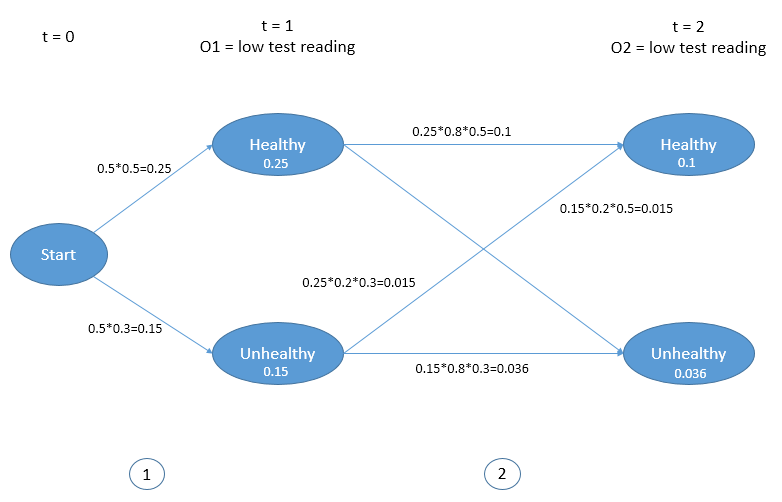
\includegraphics[scale=0.5]{./most_likely_state_sequence.png}
	\caption{Viterbi's Algorithm}
	\label{fig:most likely state sequence}
\end{figure}

The algorithm can be divided into two stages:
\\1. For the stage 1 ($t_{0}->t_{1}$), we have $P(newState)=P_{start}(state) * P_{observation}("low test reading")$. Thus, the most likely state in $t_{1}$ is Heathly (P=0.5).
\\2. For the stage 2 ($t_{1}->t_{2}$), we have $P_{newState} = P_{oldState} * P_{trans}(oldState->newState) * P_{oberservation}("low test reading" | newState)$. Thus, the most likely state in $t_{2}$ is Healthy (P=0.1).
\\As a result, the most likely state sequence for t = 0,1,2 given the evidence from the previous subpart is {Healthy, Healthy}.

\section{EM for mixtures of Bernoullis}
\paragraph{\textbf{Answer1}}
For a Bernoullis distribution models, we have P(X=x) = $\mu$ , where $x\in \left \{ 0,1 \right \}, \mu \in \left [ 0,1 \right ]$.
\\\\ For the mixture of K Bernoullis distrutions, we have $P(X=x|\mu , \pi _{k})=\sum_{k=1}^{K}\pi_{k}P(X=x|\mu _{k})$, where $\mu =\left \{ \mu _{1},...,\mu _{k} \right \}, \pi=\left \{ \pi_{1},...,\pi_{k} \right \} and P(X=x|\mu_{k})=\prod_{i=1}^{D}\mu_{k_{i}}^{x^{(i)}}(1-\mu_{k_{i}})^{(1-x^{(i)})}$. $\pi_{k}$ are the mixture proportions.
\begin{align*}
\left\{\begin{matrix}
	z^{(i)} \sim Multibernoullis(\pi); \pi_{k}>0, \sum_{k}\pi_{k}=1
	\\ 
	x^{(i)}|_{z^{(i)}=k} \sim B(\mu_{k},\sum_{k})
\end{matrix}\right.
\end{align*}
\\\\Given data set $X=\left\{x_{1},...,x_{m}\right\}$, we have the loss function and log likelihood:
\begin{align*}
&L=\prod_{i=1}^{m}P(x^{(i)}|\mu,\pi)
\\&=\prod_{i=1}^{m}\sum_{k=1}^{K}P(z^{(i)};\pi)P(x^{(i)}|z^{(i)}=k;\mu)
\end{align*}
\begin{align*}
&l=\sum_{i=1}^{m}\sum_{k=1}^{K}r_{k}^{(i)}log\frac{\left [P(z^{(i)};\pi)P(x^{(i)}|z^{(i)}=k;\mu)  \right ]}{r_{k}^{(i)}}
\\&=\sum_{i=1}^{m}\sum_{k=1}^{K}r_{k}^{(i)}\left [ \sum_{j=1}^{D}\left ( x_{j}^{(i)}log\mu_{kj}+\left ( 1-x_{j}^{(i)}log(1-\mu_{kj}) \right ) \right ) + log\pi_{k}-logr_{k}^{(i))} \right ]
\end{align*}
Thus, let the derivative equal to 0, we have
\begin{align*}
\sum_{i=1}^{m}r_{k}^{(1)}\left ( \frac{x_{j}^{(i)}}{\mu_{kj}}- \frac{1-x_{j}^{(i)}}{1-\mu_{kj}}\right )=0
\end{align*}
Finally, we can have:
\begin{align*}
\mu_{kj}=\frac{\sum_{i=1}^{m}r_{k}^{(i)}x_{j}^{(ii)}}{\sum_{i=1}^{m}r_{k}^{(i)}}
\end{align*}


\paragraph{\textbf{Answer2}}
If we have a Beta($\alpha, \beta $) prior, then we have:
\begin{align*}
P(X=x|\mu_{k})=\prod_{i=1}^{D}\mu_{k_{i}}^{\alpha - 1}(1-\mu_{k_{i}})^{\beta-1}
\end{align*}

According to the last question, we can have:
\begin{align*}
\frac{\alpha - 1}{\mu_{kj}} - \frac{\beta - 1}{1 - \mu_{kj}} + \sum_{i=1}^{m}r_{k}^{(1)}\left ( \frac{x_{j}^{(i)}}{\mu_{kj}}- \frac{1-x_{j}^{(i)}}{1-\mu_{kj}}\right )=0
\end{align*}
Finally, we can have:
\begin{align*}
\mu_{kj}=\frac{\sum_{i=1}^{m}r_{k}^{(i)}x_{j}^{(ii)} + \alpha -1}{\sum_{i=1}^{m}r_{k}^{(i)} + \alpha + \beta - 2}
\end{align*}


\section{Principal Components Analysis}
Solution: 
\\We know that V = $\left \{ \alpha u : \alpha \epsilon R \right \}$. Thus, we have:
\begin{align*}
f_{u}(v)& = argmin_{v\epsilon V}||x - v||^{2}
\\&= argmin_{v\epsilon V}(x - \alpha u)^{T}(x - \alpha u)
\\&= argmin_{v\epsilon V}(x^{T}x - \alpha^{T}u^{T}x - x^{T}\alpha u  + u^{T}u \alpha^{2})
\end{align*}
To get the minimum of $f_{u}(v)$, we can let its derivative equal to 0, so we have:
\begin{align*}
\frac{\partial f_{u}(v)}{\partial  \alpha}&=-2u^{T}x + 2\alpha = 0
\end{align*}
Then we have:
\begin{align*}
\alpha = u^{T}x
\end{align*}
Thus
\begin{align*}
f_{u}(v)=u^{T}xu
\end{align*}
After that, we can have:
\begin{align*}
&argmin_{u:u^{t}u=1}\sum_{i=1}^{m}||x^{(i)}-f_{u}(x^{(i)})||^{w}
\\&=argmin_{u:u^{t}u=1}\sum_{i=1}^{m}\left ( x^{(i) }- u^{T}xu \right )^{T}\left (  x^{(i) }- u^{T}xu\right )
\\&=argmin_{u:u^{t}u=1}\sum_{i=1}^{m}\left ( x^{(i)^{T}}x^{(i)} -  \left ( u^{T}x{(i)} \right )^{2}\right )
\\&=argmax_{u:u^{t}u=1}\sum_{i=1}^{m}\left (\left ( u^{T}x{(i)} \right )^{2} \right )
\end{align*}

According to the assumption that the data have zero-mean and unit variance in each dimension, so we have:
\begin{align*}
&argmin_{u:u^{t}u=1}\sum_{i=1}^{m}||x^{(i)}-f_{u}(x^{(i)})||^{w}
\\&=argmax_{u:u^{t}u=1}\sum_{i=1}^{m}\left (\left ( u^{T}x{(i)} \right )^{2} \right )
\\&=argmax_{u:u^{t}u=1}\sum_{i=1}^{m}\left (\left ( u^{T}x{(i)} - u^{T} \overline{x^{(i)}}\right )^{2} \right )
\end{align*}

So $argmin_{u:u^{t}u=1}\sum_{i=1}^{m}||x^{(i)}-f_{u}(x^{(i)})||^{w}$ can be changed to maximize the variance projected data on u, which means that it can find the principal component of the data.
\end{document}

